\documentclass[]{standalone}
\usepackage{mathptmx}
%\renewcommand{\familydefault}{\rmdefault}
\usepackage[T1]{fontenc}
\usepackage[latin9]{inputenc}
\usepackage{siunitx}
\usepackage{array}
\usepackage{amsmath}
\usepackage{ifthen}
\usepackage{pgfplots}
\usepackage{pgfmath}
\pgfplotsset{compat=1.14}
\usepackage{titling, graphicx}
\usepackage{tikz}
\usepackage{upgreek}
\usepackage{amsmath,amsthm}
\usepackage{strtikz}
\usetikzlibrary{shapes,arrows.meta,intersections,graphs,graphs.standard,math,fit}
\usetikzlibrary{calc,intersections,through,backgrounds}
\usetikzlibrary{decorations.pathmorphing, decorations.markings,decorations.pathreplacing}


\begin{document}
\begin{tikzpicture}
\lumpedmass[number of storys=3,
story height=1.0cm,
startX=0cm,
startY=0cm,
frame line thickness = 1.2pt,
support width = 0.3cm,
support height = 0.2cm,
support line thickness = 1.5pt,
show supports = 4,
isolator width = 0.5cm,
isolator thickness = 0.2cm,
isolator line thickness = 1pt,
foundation thickness = 0.3cm,
foundation width=1.2cm,
mass radius = 4pt,
show mass = 1,
show axes=0,
base slab width=0.8cm,
base slab height=0.2cm,
x axis length=0.5cm,
y axis length=0.5cm,
drift distance=0.4cm,
drift curve ratio=0.65,
base slab drift=1.15cm,
foundation drift=1.9cm,
arrow tip length=3pt,
arrow tip width=2pt,
story to place superstructure dof=2,
text for the superstructure dof=$x_i(t)$,
text for the isolation dof=$x_b(t)$,
text for the ground dof=$x_g(t)$,
text for the story mass=$m_i$,
text for the base slab mass=$m_b$,
text for the story properties={$k_i,c_i$}]
\end{tikzpicture}
\end{document}